\chapter{Modeling  the heterogeneity of the Dox-induced GFP (or mCherry) expressions} % Main chapter title

\label{Part3_chapter} % For referencing the chapter elsewhere, use \ref{Chapter1} 

\section{The model}
In order to access the heterogeneity of Dox-induced single-cell expressions in both feedback and no-feedback systems, we model the random fluctuation in biochemical reactions, random copy number variation and random epigenetic inheritance in expression systems.

\subsection{Random epigenetic inheritance}

Random epigenetic inheritance also plays an important part of fluctuation in cell population. I incorporate random epigenetic inheritance on single cell level. Epigenetic regulations, including DNA methylation, histone modification and others, influence gene expression by regulating chromatin accessibility and the interaction between DNA and protein. In the model, the reaction constants of each transcription was influenced by a random variable $\mu$ which subscribes to normal distribution.

Where:

\begin{equation} 
\begin{aligned} 
\centering
% \underset{A}{B}
% \overset{…}{…}
K_{real}   &= K_{deterministic} \times (1+\mu_1) \\
k_{d-real} &= k_{d-deterministic} \times (1+\mu_2) \\
r_{real}   &= r_{deterministic} \times (1+\mu_3) \\
\beta_{real}   &= \beta_{deterministic} \times (1+\mu_4) \\
\end{aligned} 
\end{equation}

\subsection{Random copy number variance}

Random copy number variance is an important source of noise in cell population. We incorporate random copy number variation on single cell level. In the modeling, the copy number was considered in the $\alpha$, which was influenced by a random variable $\tau$ which subscribes to normal distribution.

Where:

\begin{equation} 
\begin{aligned} 
\centering
% \underset{A}{B}
% \overset{…}{…}
\alpha_{real}   &= \alpha_{deterministic} \times (1+\tau) \\
\end{aligned} 
\end{equation}

\subsection{Random basal expression level of GFP, mCherry and tetR-dimer}

Random copy number variance is an important source of noise in cell population. We incorporate random copy number variation on single cell level. In the modeling, the basal expression level of GFP, mCherry and free tetR-dimer were influenced by a random variable $\xi$ which subscribes to normal distribution.

Where:

\begin{equation} 
\begin{aligned} 
\centering
% \underset{A}{B}
% \overset{…}{…}
[GFP]_{0-real}   &= [GFP]_{0-deterministic} \times (1+\xi_1) \\
[mCherry]_{0-real}   &= [mCherry]_{0-deterministic} \times (1+\xi_2) \\
[R^2_0]_{0-real}   &= [R^2_0]_{0-deterministic} \times (1+\xi_3) \\
\end{aligned} 
\end{equation}

%----------------------------------------------------------------------------------------
\section{Simulate the flow cytometry data with simulations of 1000 cells}

Combing the factors of random fluctuation in biochemical reactions, random copy number variance and random epigenetic inheritance described above, we establish model to study the heterogeneity of Dox-induced single-cell expressions in both feedback and no-feedback systems. For each doxycycline concentration, we stimulate 1000 single cells.

\subsection{Heterogeneity of Dox-induced single-cell expressions, without feedback}

For the heterogeneity of Dox-induced single-cell expressions of GFP without feedback, the stimulation result is as follows:

\begin{figure}[H]
\centering
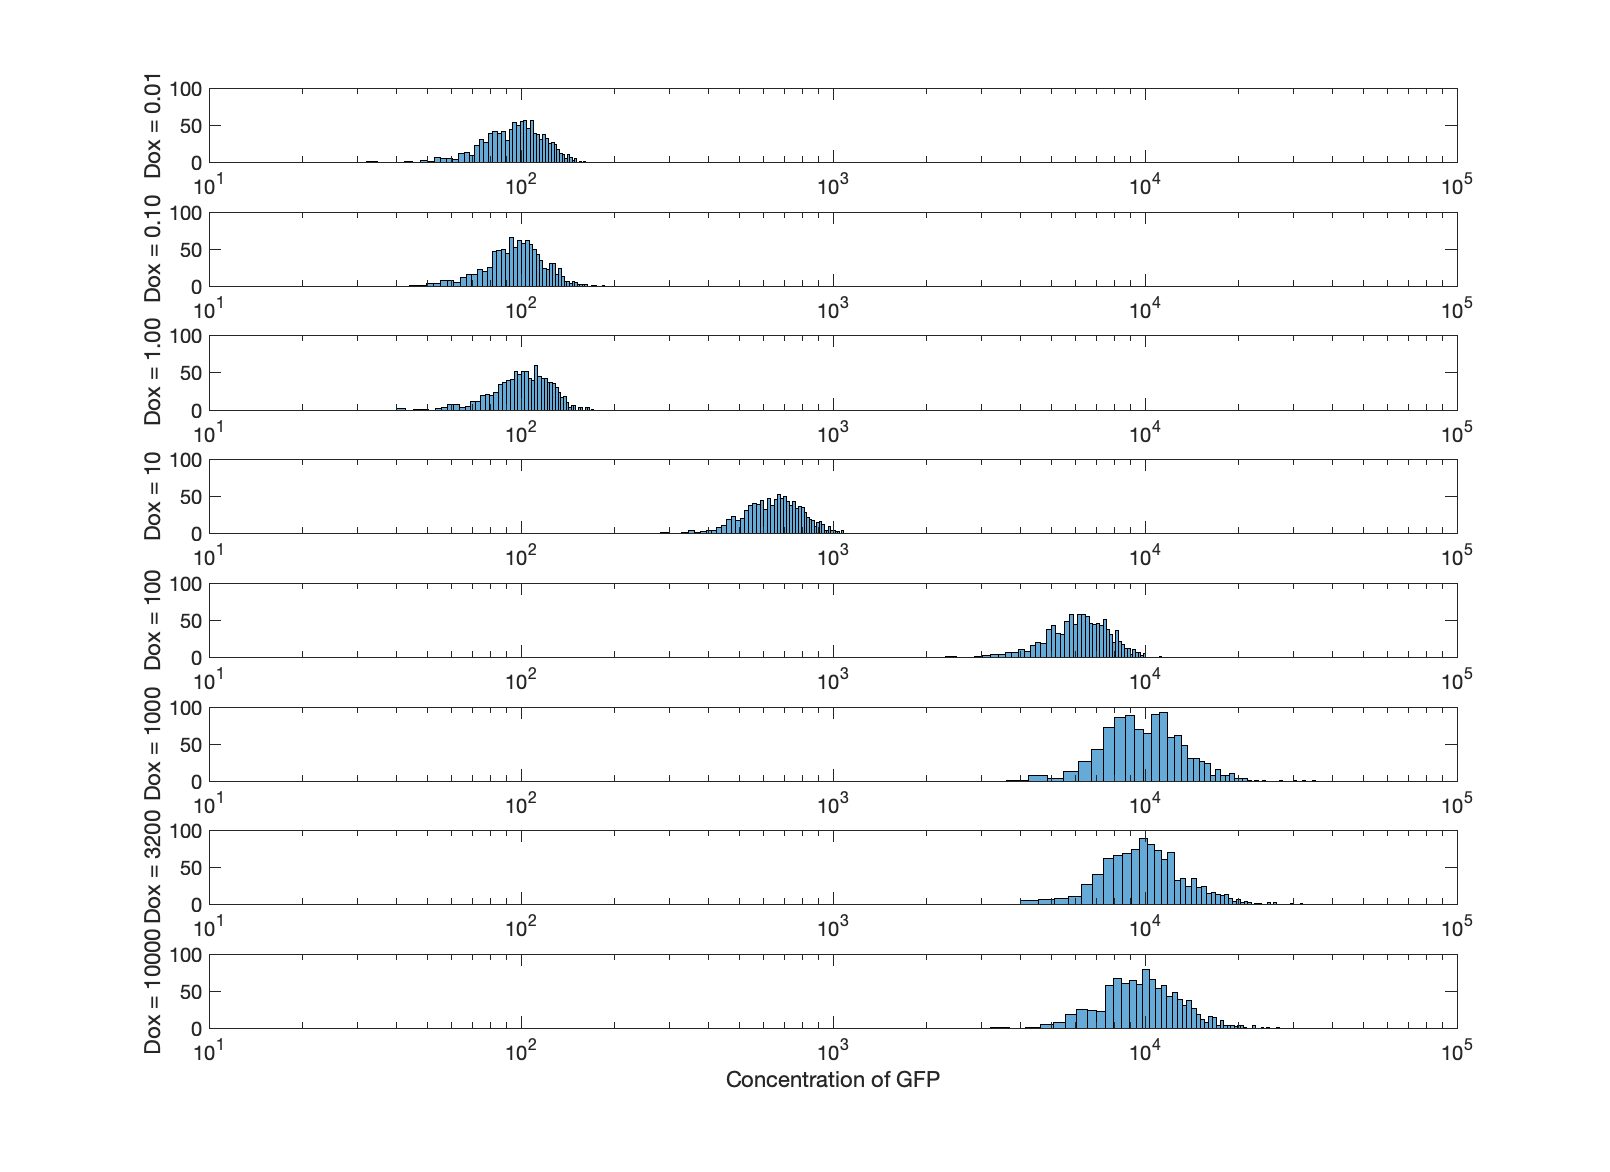
\includegraphics[width=1.0\linewidth]{Figures/Q3_1.png}
\caption{Cytometry simulations of Dox-induced GFP expression \\ system without feedback in 1000 cells}
\label{part_3_1}
\end{figure}

From the figure we can see that for each concentration of doxycycline, the GFP expression in cell population is like a normal distribution. At low concentration of doxycycline, increasing doxycycline concentration would not cause much to distribution of GFP expression, this is because at this stage there is surplus of tetR dimer in addition to binding most of tetO. At higher concentration of doxycycline, increasing doxycycline concentration would not cause much change to the distribution of GFP expression, this is because at this stage the doxycycline is enough to bind most of the tetR dimer.

\subsection{Heterogeneity of Dox-induced single-cell expressions, with feedback}

For the heterogeneity of Dox-induced single-cell expressions of mCherry with feedback, the result is as follows:

\begin{figure}[H]
\centering
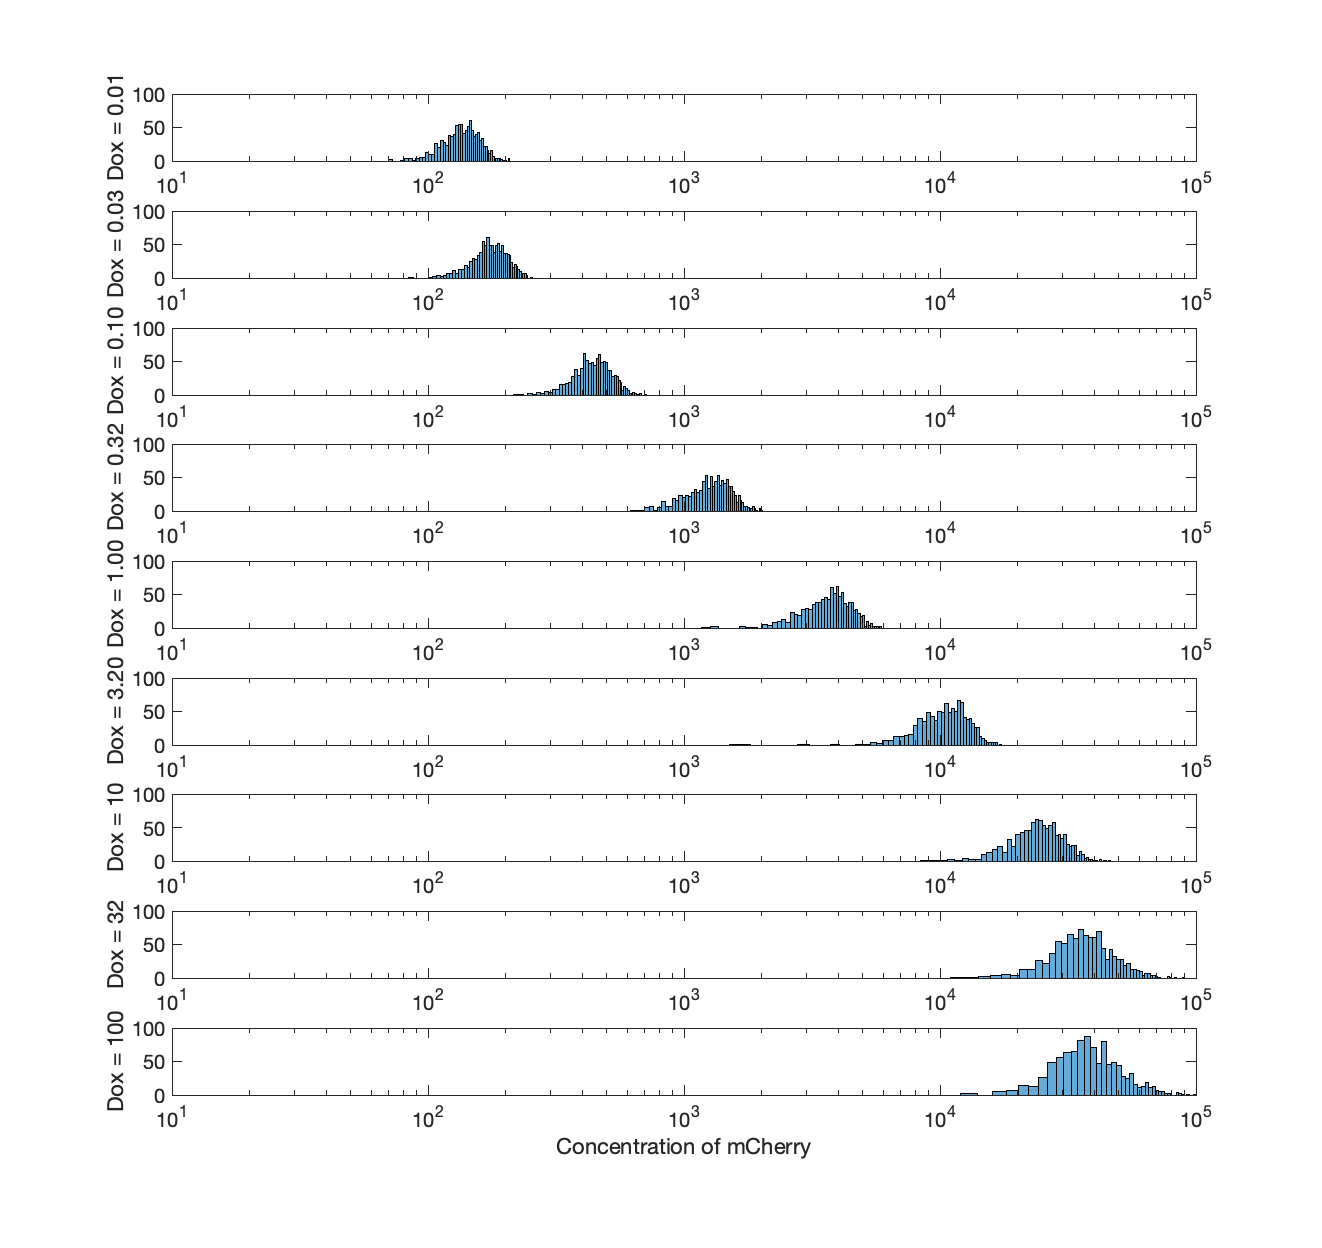
\includegraphics[width=1.0\linewidth]{Figures/Q3_2.png}
\caption{Cytometry simulations of Dox-induced mCherry expression \\system with feedback in 1000 cells ($log10 \approx 3.2$)}
\label{part_3_2}
\end{figure}

From the figure we can see that for each concentration of doxycycline, the mCherry expression in cell population is like a normal distribution. As the concentration of doxycycline increase, the mean of mCherry expression show a steady increase. This is because there is a negative feedback control loop in this system, increasing the concentration of doxycycline will always lead to the system to reach a new equilibrium.

%----------------------------------------------------------------------------------------
\newpage
\section{Discussion}
In this session, we discuss the result and compare our results with the experiment result.

For part1, our result looks very similar to the experiment result, including the initial value, the end value and the turning point. At low concentration of doxycycline, increasing doxycycline concentration would not cause much difference to GFP expression, this is because at this stage there is surplus of tetR dimer in addition to binding most of tetO. At higher concentration of doxycycline, increasing doxycycline concentration would not cause much to GFP expression too, this is because at this stage the doxycycline is enough to bind most of the tetR dimer. This system is responsive to doxycycline only in a narrow range of doxycycline concentration, and the response is ultrasensitive.

For part2, our result also looks very alike to the experiment result, including the initial value and the end value. As the concentration of doxycycline increase, the mean of mCherry expression show a steady increase. This is because there is a negative feedback control loop in this system, increasing the concentration of doxycycline will always lead to the system to reach a new equilibrium. This system is sensitive to a wide range doxycycline and it is easy to tune to achieve precise and quantitate control mCherry expression.

We combine the result of part1 and part2 together, the result is as follows:

\begin{figure}[H]
\centering
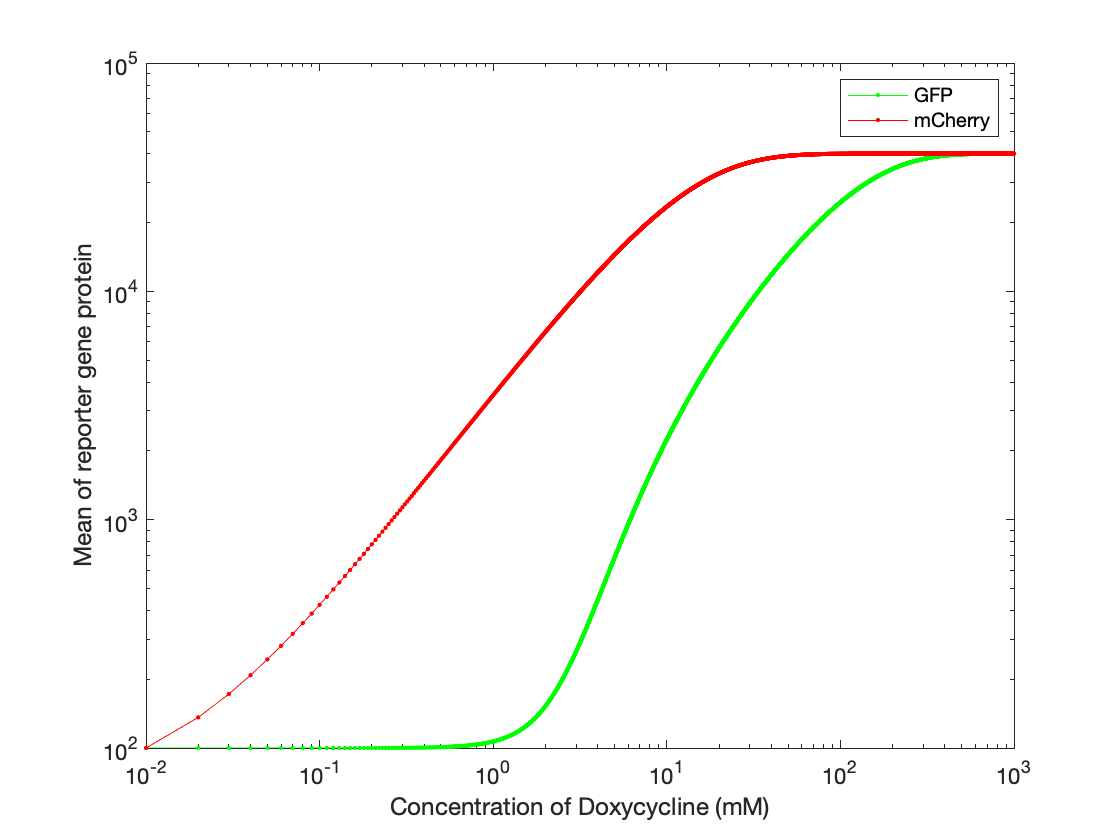
\includegraphics[width=0.8\linewidth]{Figures/Q3_3.png}
\caption{The modeling results for GFP without feedback \\ and mCherry with feedback}
\label{part_3_3}
\end{figure}

The system without feedback is ultrasensitive to doxycycline in a narrow concentration range, while the system with feedback is sensitive to a wide range doxycycline and it is easy to tune to achieve precise and quantitate control mCherry expression. The difference is due to the feedback control: It can control the equilibrium of the reaction and stabilize the system, thus the system with feedback is responsive to wider range of doxycycline concentration, and increasing the concentration of doxycycline will lead to gentle change in target gene expression.

For part3, our modeling result of the system without feedback has similar mean value of the distribution comparing with the experiment result. But at higher concentration of doxycycline, the distribution of experiment result has heavier tail than our modeling result. We hypothesis that the difference is due to some unknown biological pathways. For instance, at higher concentration of doxycycline, some other biological pathways are affected thus lead to the heavier tail in the distribution of experiment result. In addition, our modeling result of system with feedback is similar to the experiment result, both in mean value and distribution shape.

